\documentclass[a4paper,12pt]{report}
\usepackage{graphicx}
\usepackage{pdfpages}
\usepackage{algorithm}
\usepackage{algorithmic}
\usepackage{labelcas}

\usepackage{listings}
\usepackage{color}

\definecolor{dkgreen}{rgb}{0,0.6,0}
\definecolor{gray}{rgb}{0.5,0.5,0.5}
\definecolor{mauve}{rgb}{0.58,0,0.82}

\lstset{frame=tb,
  aboveskip=3mm,
  belowskip=3mm,
  showstringspaces=false,
  columns=flexible,
  basicstyle={\small\ttfamily},
  numbers=none,
  numberstyle=\tiny\color{gray},
  keywordstyle=\color{blue},
  commentstyle=\color{dkgreen},
  stringstyle=\color{mauve},
  breaklines=true,
  breakatwhitespace=true
  tabsize=3
}

\begin{document}

\chapter{Analysis}

\section{Introduction}

\subsection{Client Identification}

My client is Josh Campbell, he is 24 years old. He uses computers regularly for deisgn work, so has experience of computer systems. He uses his computer to design flyers, handouts, banners and visual graphics for projection, as well as surfing the web, email and various social media networks.He rarely uses hard copies other than to preview hes work before sending it off to print. Josh uses a 2012 Mac Pro with the latest version of Apple's operating system, OS X (10.9).

Josh is the head of the media department for Cambridge Community Church. This involves being responcible for the large amount of Audio and Visual equipment used on the churches Sunday services. This currently invloves spreadsheet with limited info on each item. 

Josh would like to have a database management system to be able to hold information about each item and their various attributes. He would likke this database to be lovated on the churches central server so that it can be accessed by all staff if it it deemed necessary. He would use this database to store location, value and insurance details incase of damage or theft.he would like all of the information kept as a virtual copy as well as a hard copy to kept as a visual backup in case of harddrive failure or corruption. He would also like to keep the location of each item as up to date as possible and if the location changes, he would like to be notified by email when it is entered/updated in the system.

\subsection{Define the current system}

The current system consists of multiple excel spreed sheets. There is one spread sheet for each of three locations; main office, main church building, and storage. Each spreedsheet consists of items located there as well as information on the value of each item, the quantity and the total value for the items with multiple entries. Each spreedsheet is divided up into equipment type (i.e Cableing, lighting, audio, visual/camera's) 

\subsection{Describe the problems}

There are a number of problems with the current system. One of the problems is that there is no notification system to tell you when information is getting outdated or something is changed. For example, if an item is bought or sold, the total costings for that item will be updated and no-one will be notified. Another problem is that the current system doesn't show the PAT testings for all the items, these tests go out of date every 6 months and there is no way of being notified when a new PAT test is needed on an item.

\subsection{Section appendix}

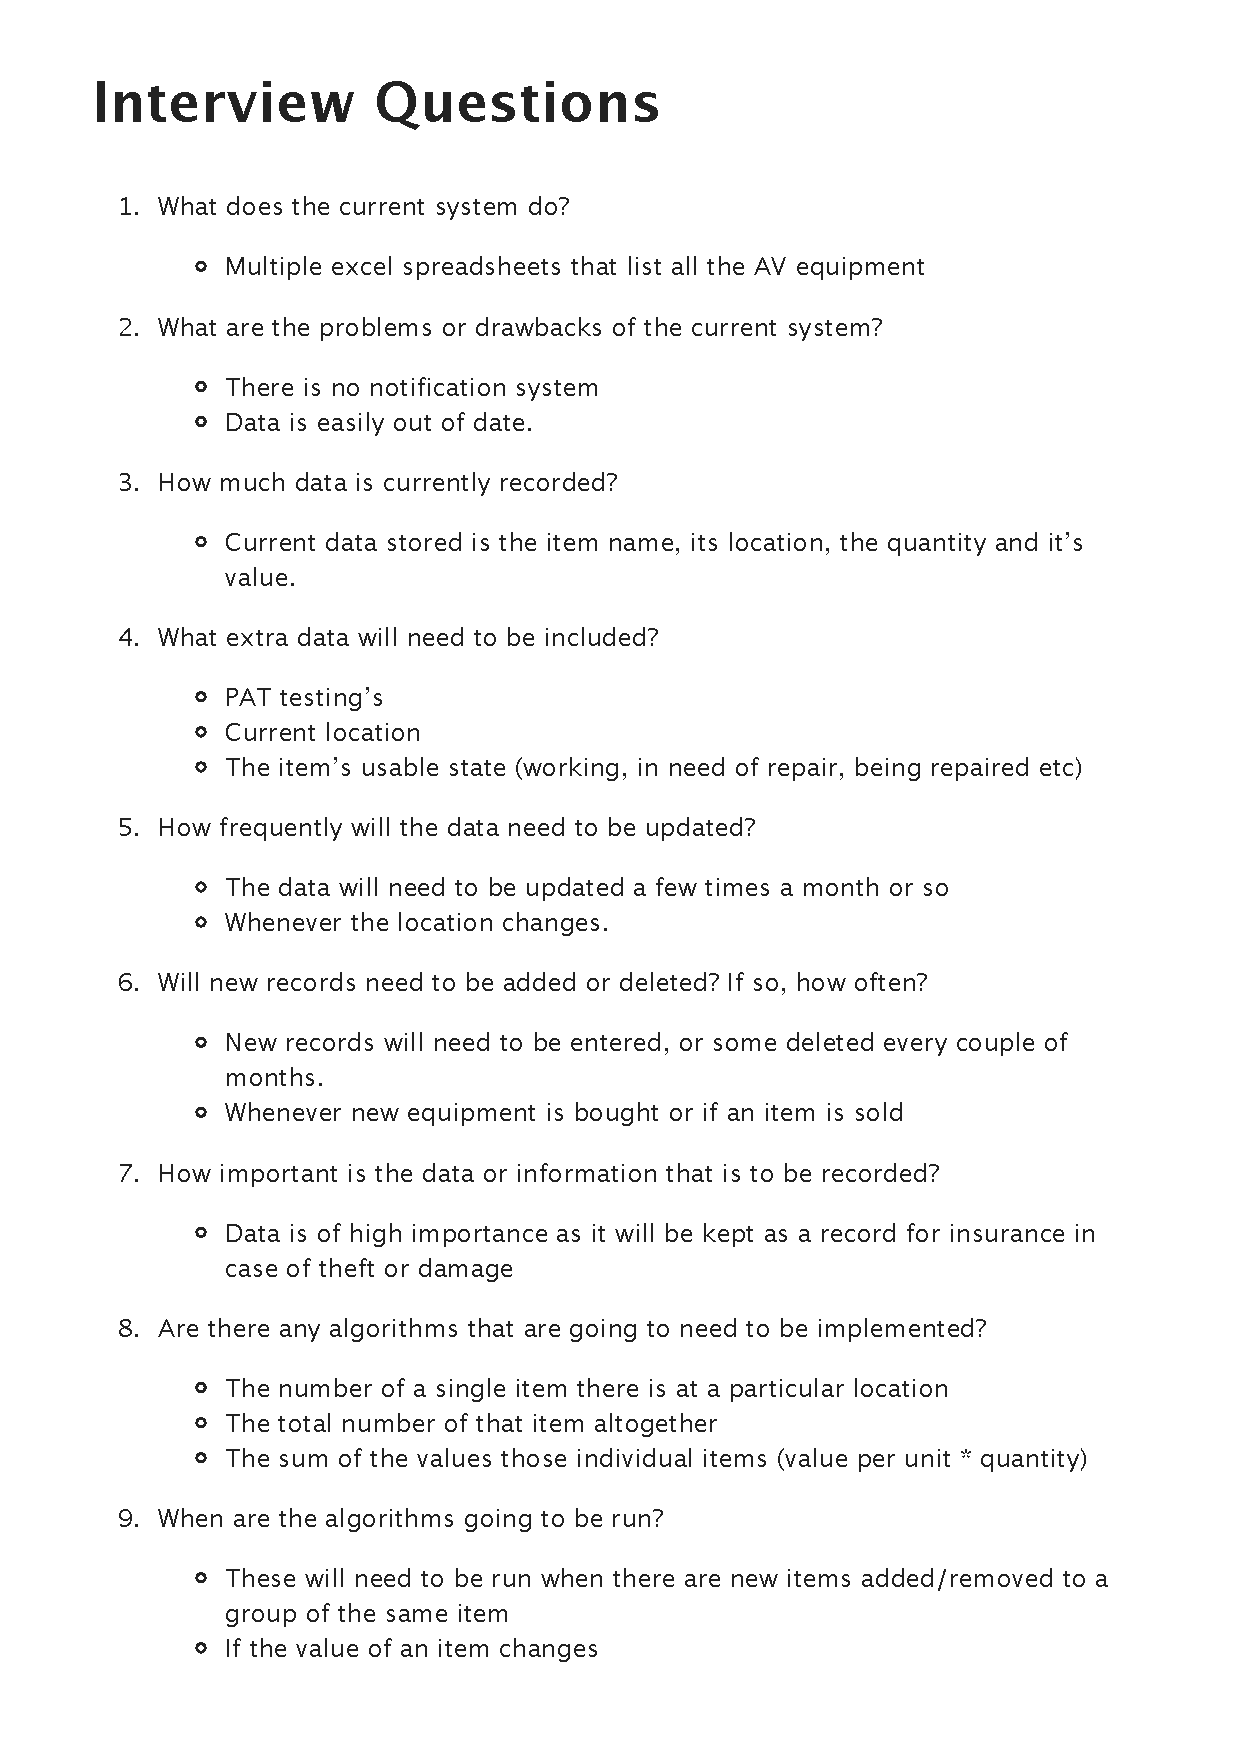
\includepdf[pages=-]{./Interview/interview_questions.pdf}

\section{Investigation}

\subsection{The current system}

\subsubsection{Data sources and destinations}

In the current system, there are multiple data sources. The client and his colleagues as well as members of the AV crew for the church can enter data into the spreadsheet by using a computer in the office and accessing the on the server.

\subsubsection{Algorithms}

In the current system, there are only a few algorithms in place.
\bigskip

Algorithm 1, When new item is bought:
\begin{lstlisting}
IF Item = NewItem DO
        Enter Item into Spreadsheet
    ELIF Item = ItemMatch Do
        Update Item Quantity
\end{lstlisting}
\bigskip

Algorithm 2, When an item is sold or replaced:
\begin{lstlisting}
IF Item = Sold OR Item = Damaged or Item = Stolen DO
    Update Quantity
    IF Item = Stolen OR Item = Damaged DO
        Claim Insurance
\end{lstlisting}

\subsubsection{Data flow diagrams}

\begin{figure}[H]
    \caption{Flow Diagram Key.} \label{fig:print_function_result}
    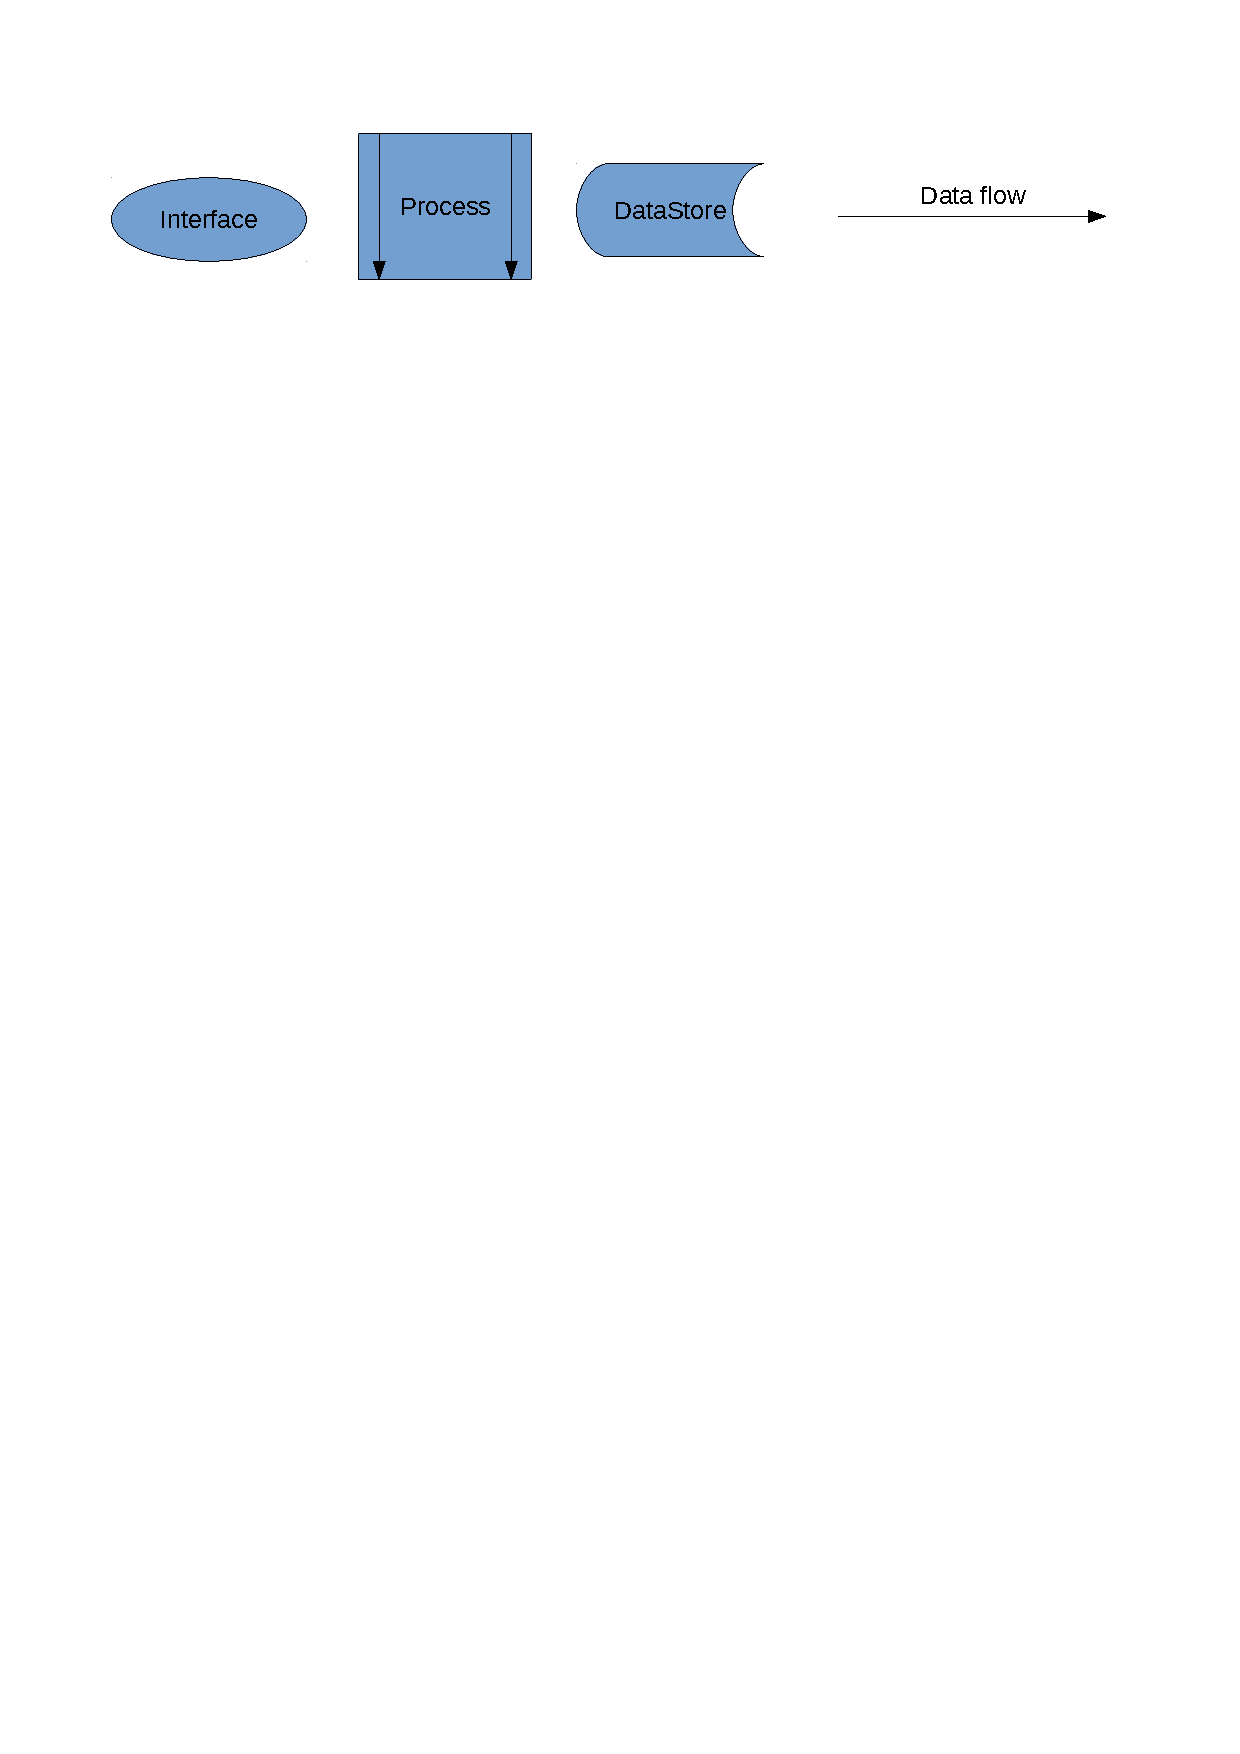
\includegraphics[width=\textwidth]{./Dataflow/DFD_analysis_key.pdf}
\end{figure}

\begin{figure}[H]
    \caption{Entering a new item.} \label{fig:print_function_result}
    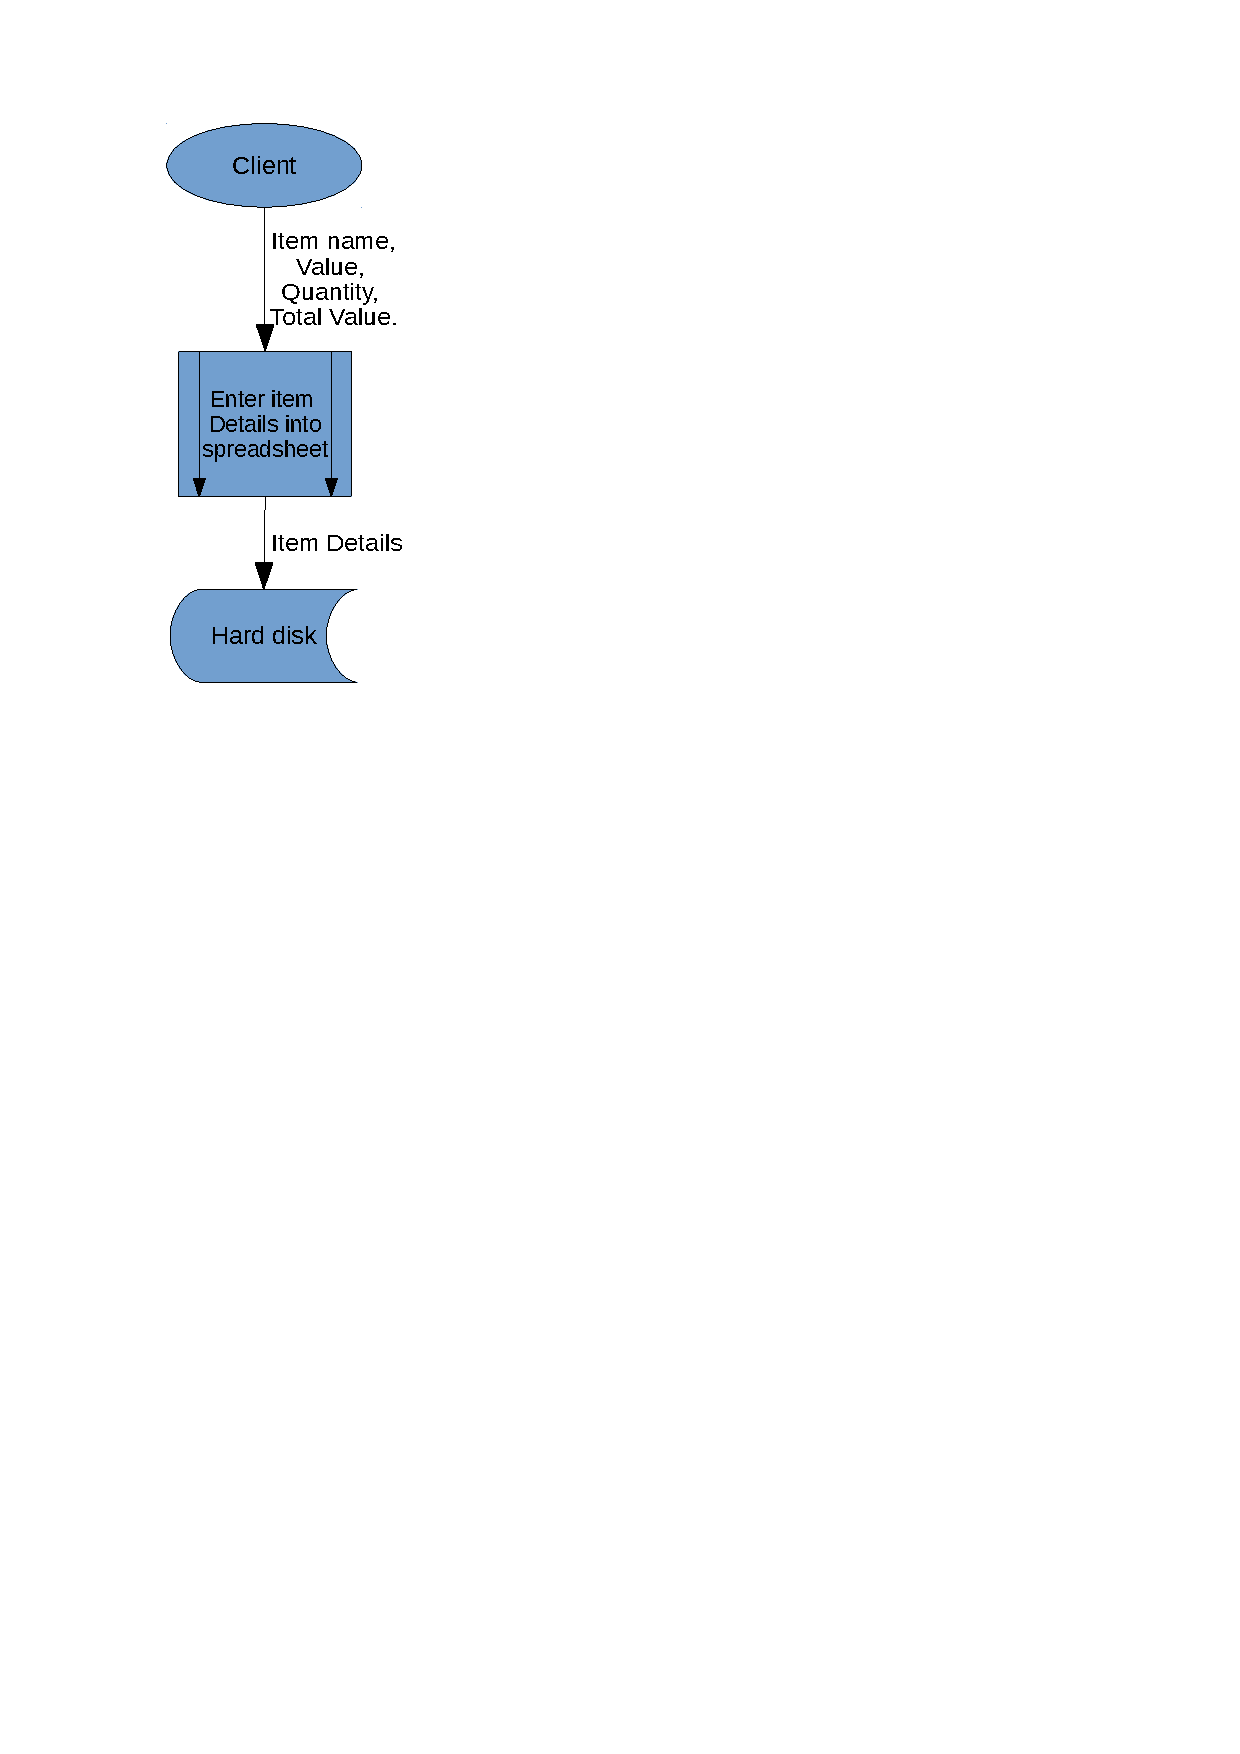
\includegraphics[width=125px]{./Dataflow/DFD_analysis_new_item.pdf}
\end{figure}

\begin{figure}[H]
    \caption{Flow Diagram Key.} \label{fig:print_function_result}
    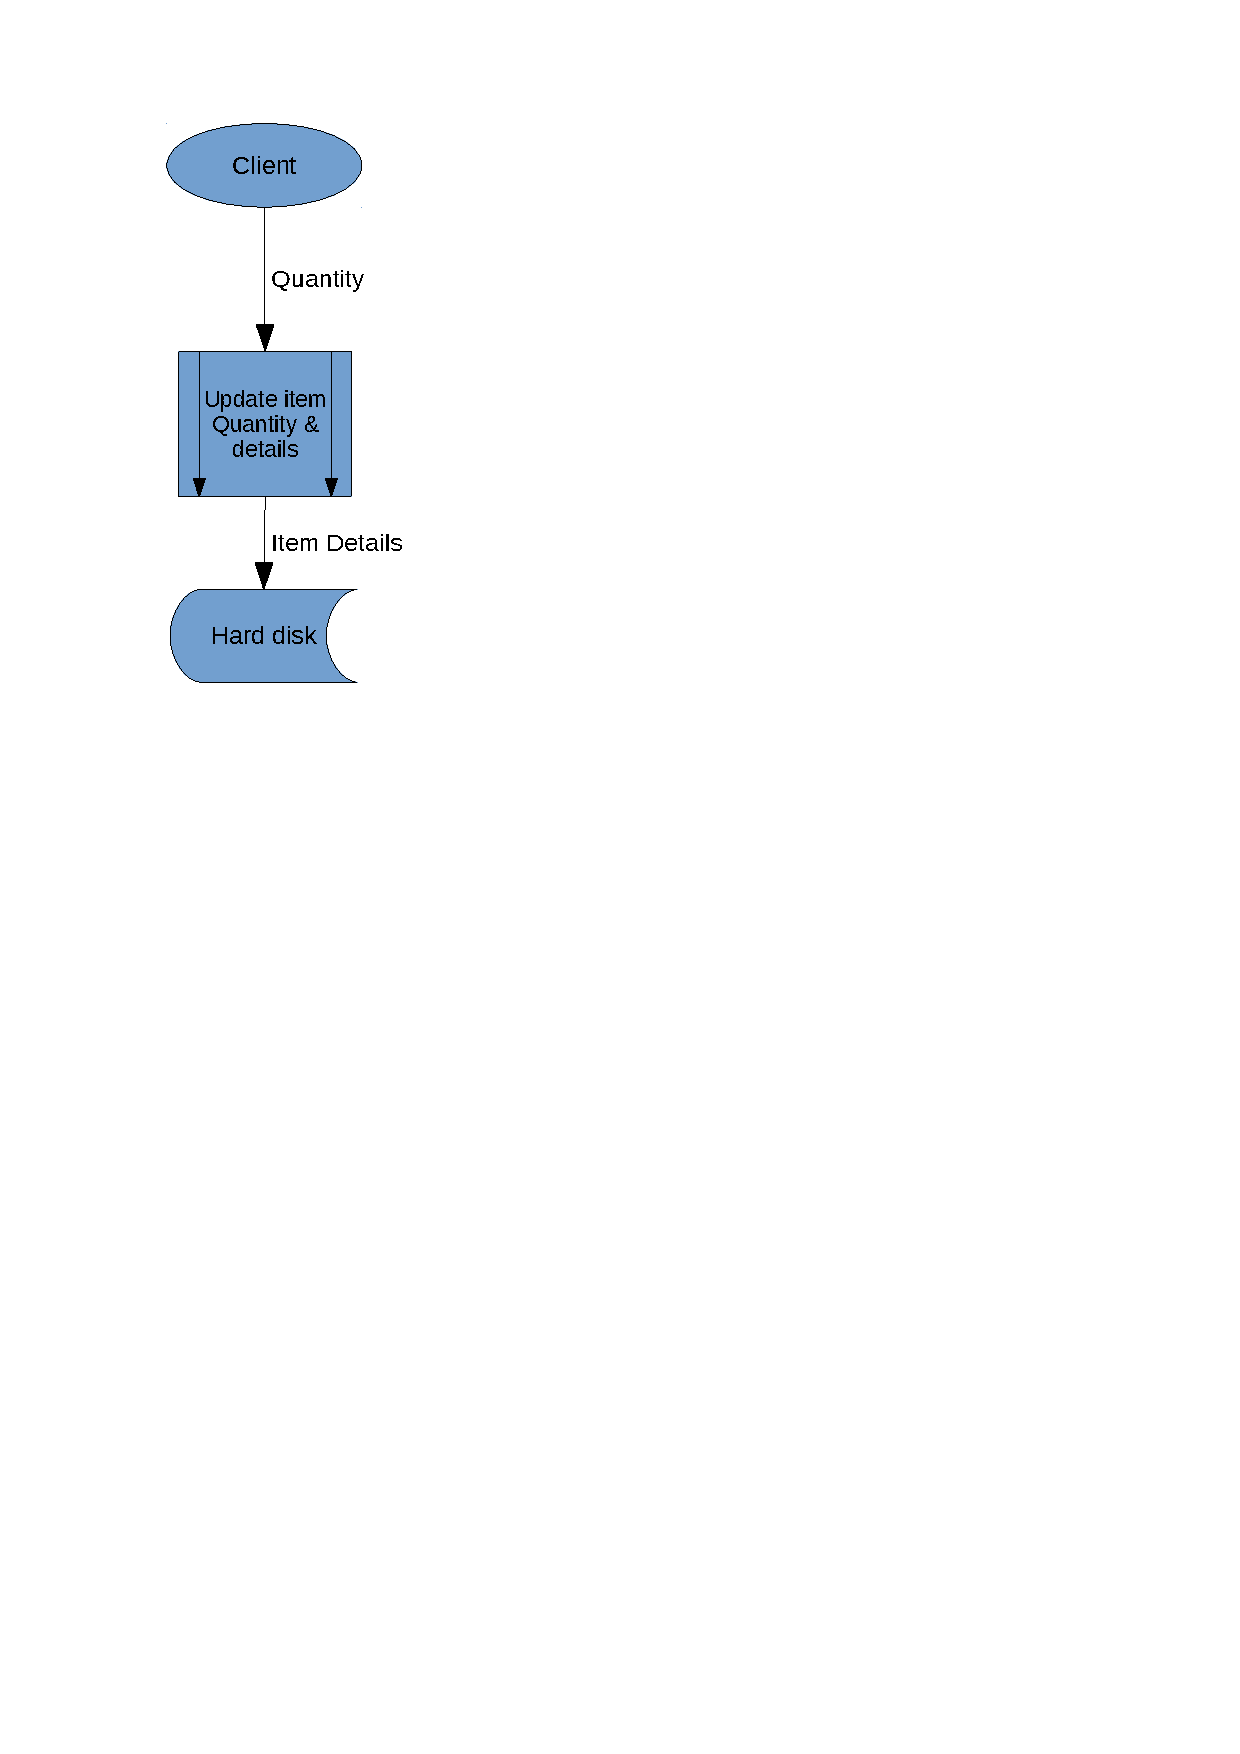
\includegraphics[width=125px]{./Dataflow/DFD_analysis_update_item.pdf}
\end{figure}

\newpage

\subsubsection{Input Forms, Output Forms, Report Formats}

Josh's current system only has one input form, this is an electronic form which is the application excel. Josh also has two ouput forms - an invoice form for when he hires out equipment to a third party and a quote sheet to show the value of a piece of equipment when he needs to insure it.

Below is an example of the input method used to insert data into the current system.




Below is an example of one of Josh's Invoice forms. The headings show Product Name, Loan Rate, Length of Loan and Total Cost.

Here is an example of a quote sheet that Josh has given me.

\newpage

\subsection{The proposed system}

\subsubsection{Data sources and destinations}

The Following table shows the proposed data and their respective sources and destinations.

\begin{figure}[H]
    \caption{Data sources and destinations} \label{fig: Data sources and destinations}
    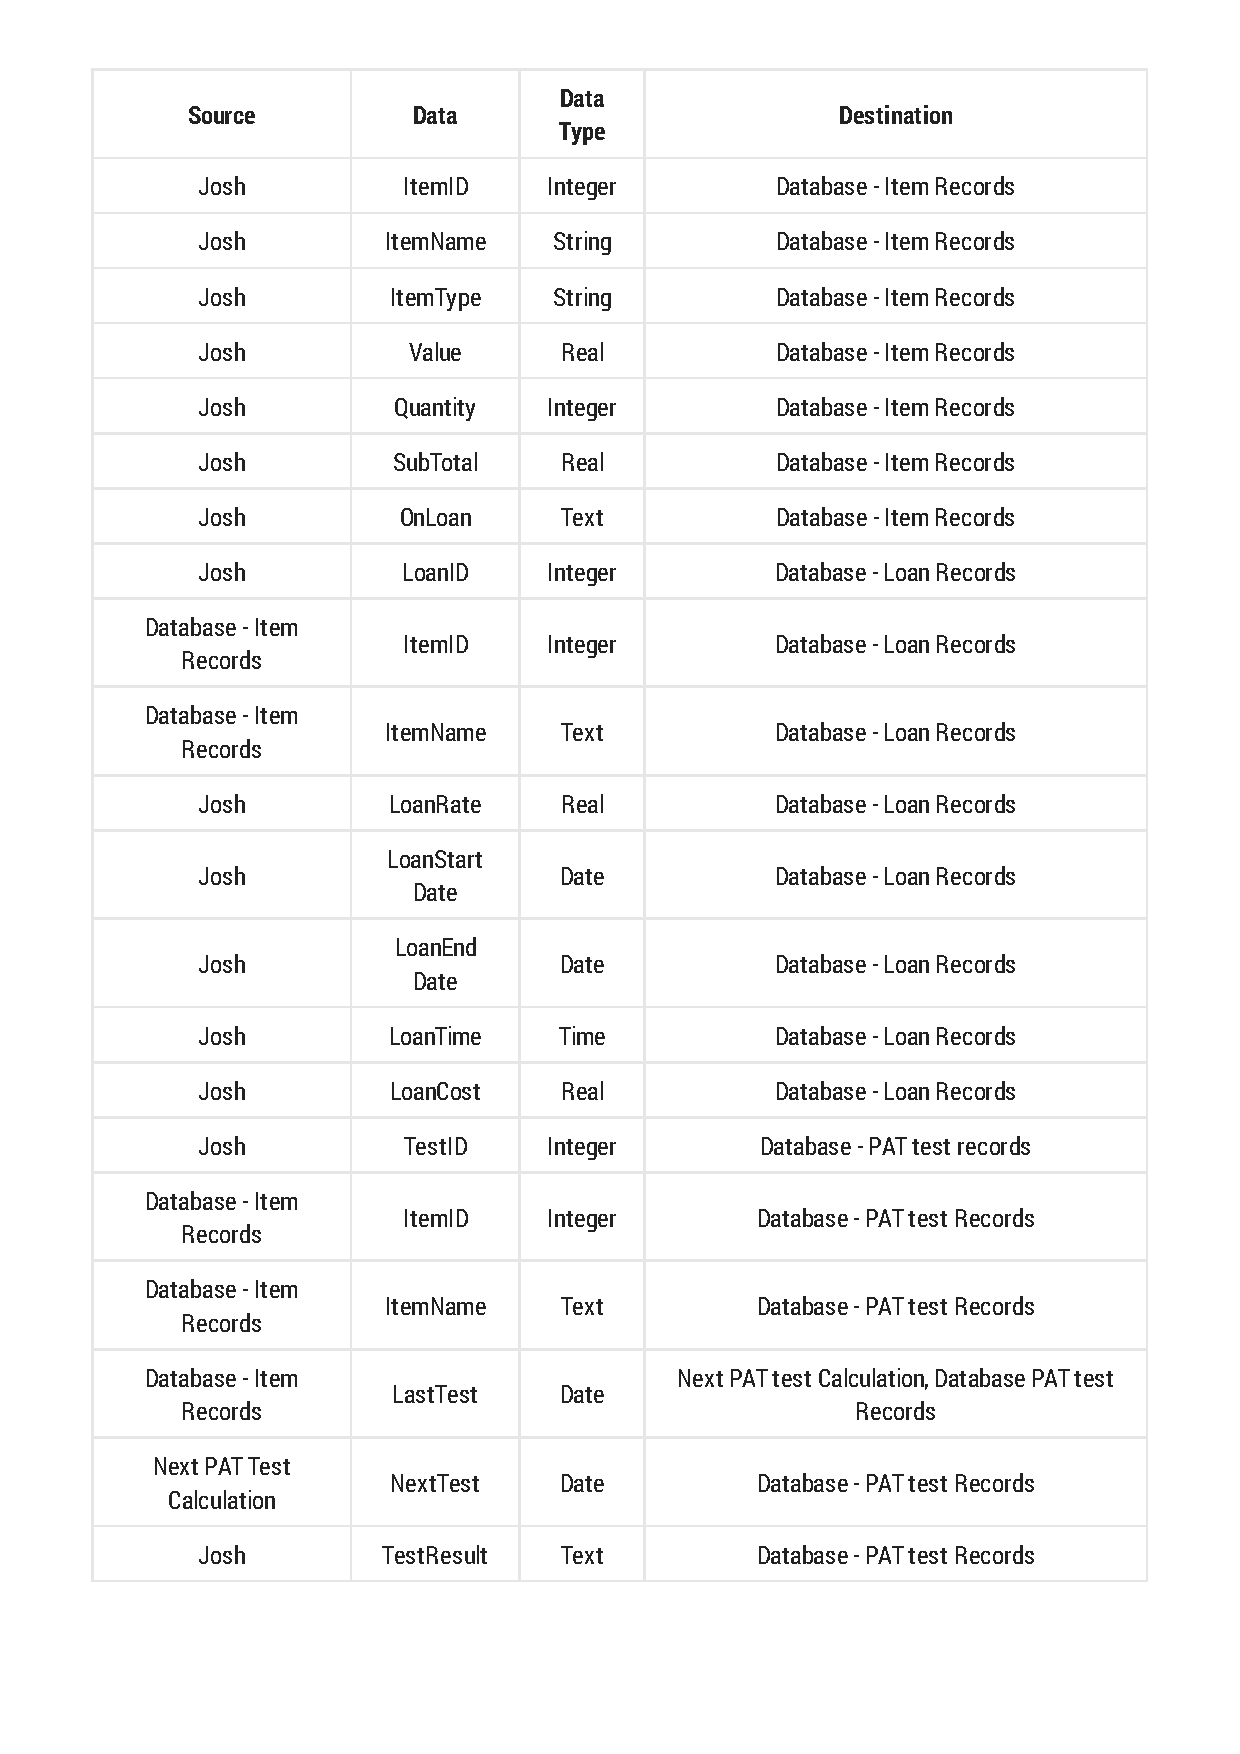
\includegraphics[page=1,width=380px]{./DataS&D/Data_S&D.pdf}
\end{figure}

\subsubsection{Data flow diagram}

\begin{figure}[H]
    \caption{Flow Diagram Key.} \label{fig:print_function_result}
    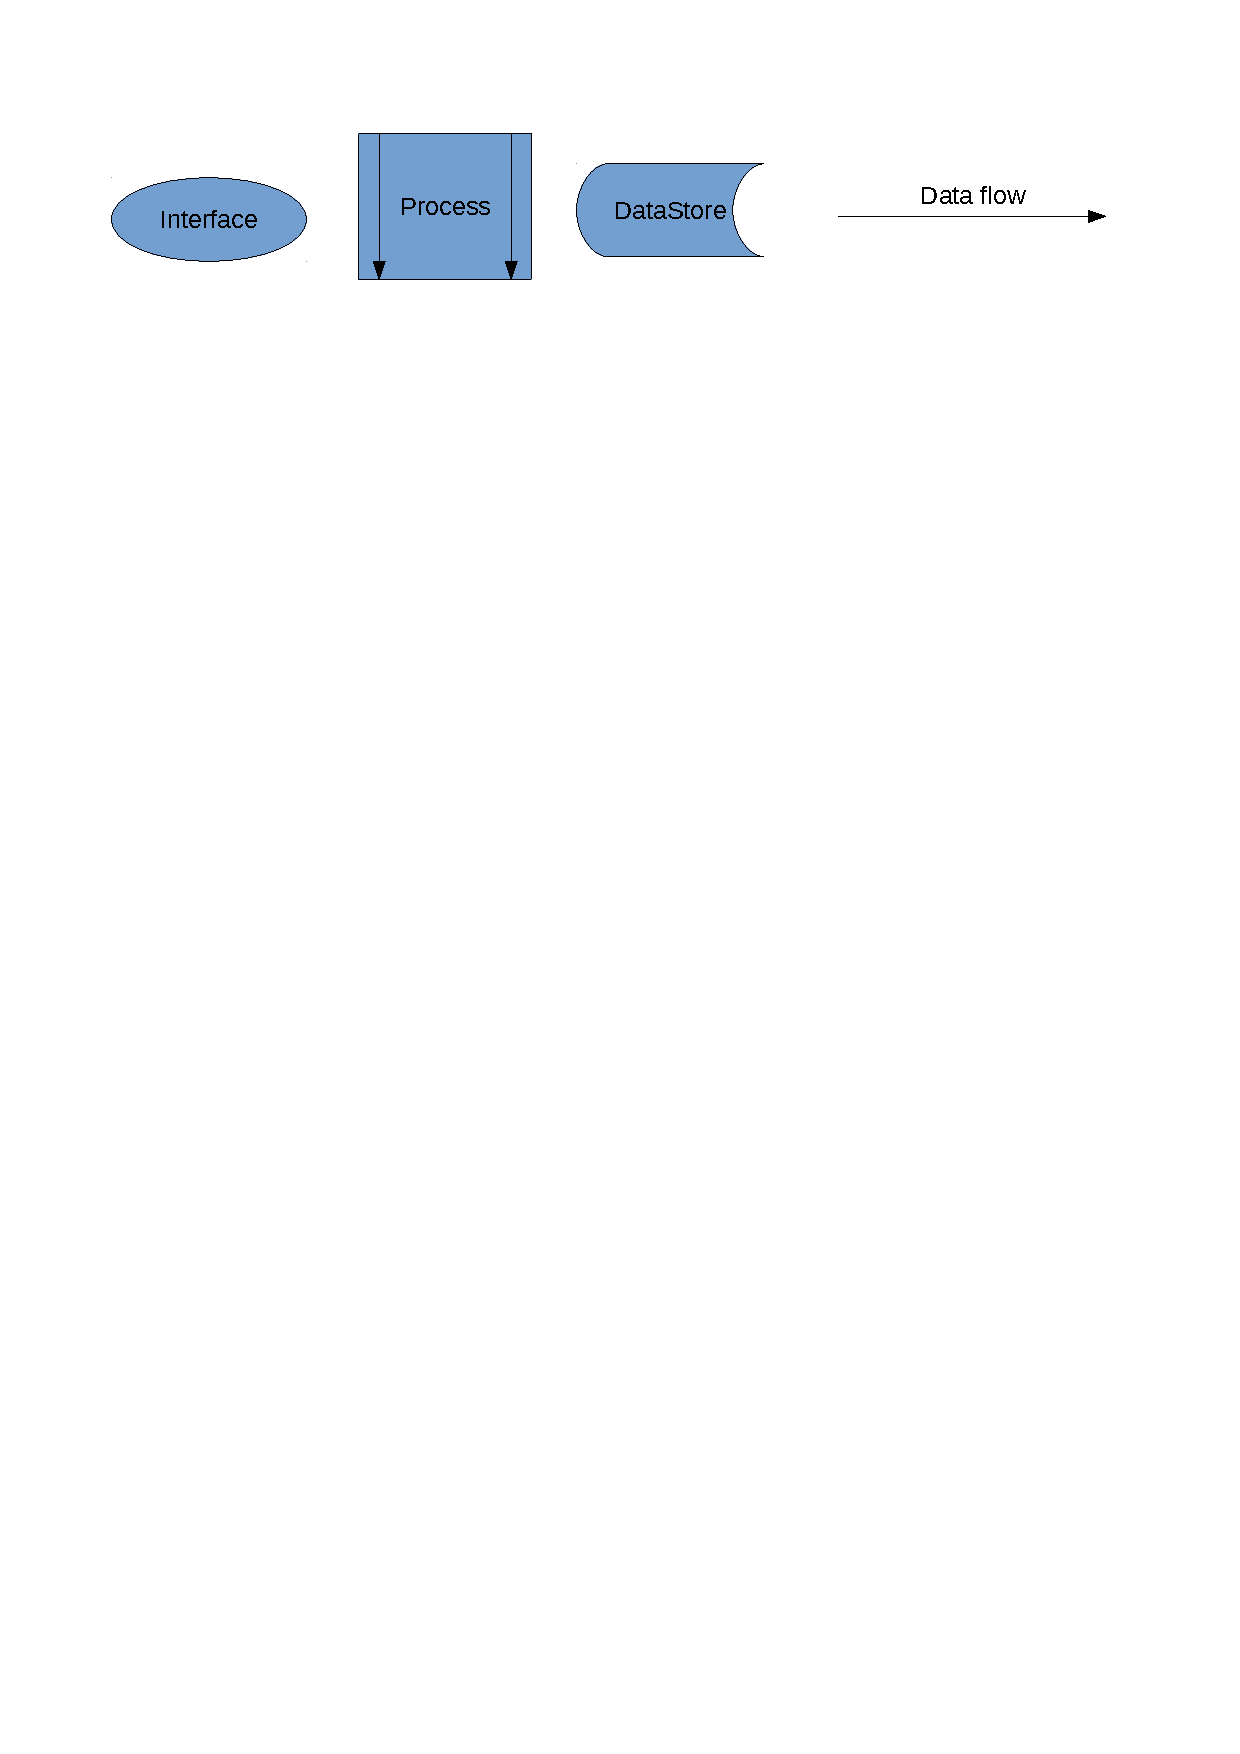
\includegraphics[width=\textwidth]{./Dataflow/DFD_analysis_key.pdf}
\end{figure}

\begin{figure}[H]
    \caption{Enter New Item.} \label{fig:print_function_result}
    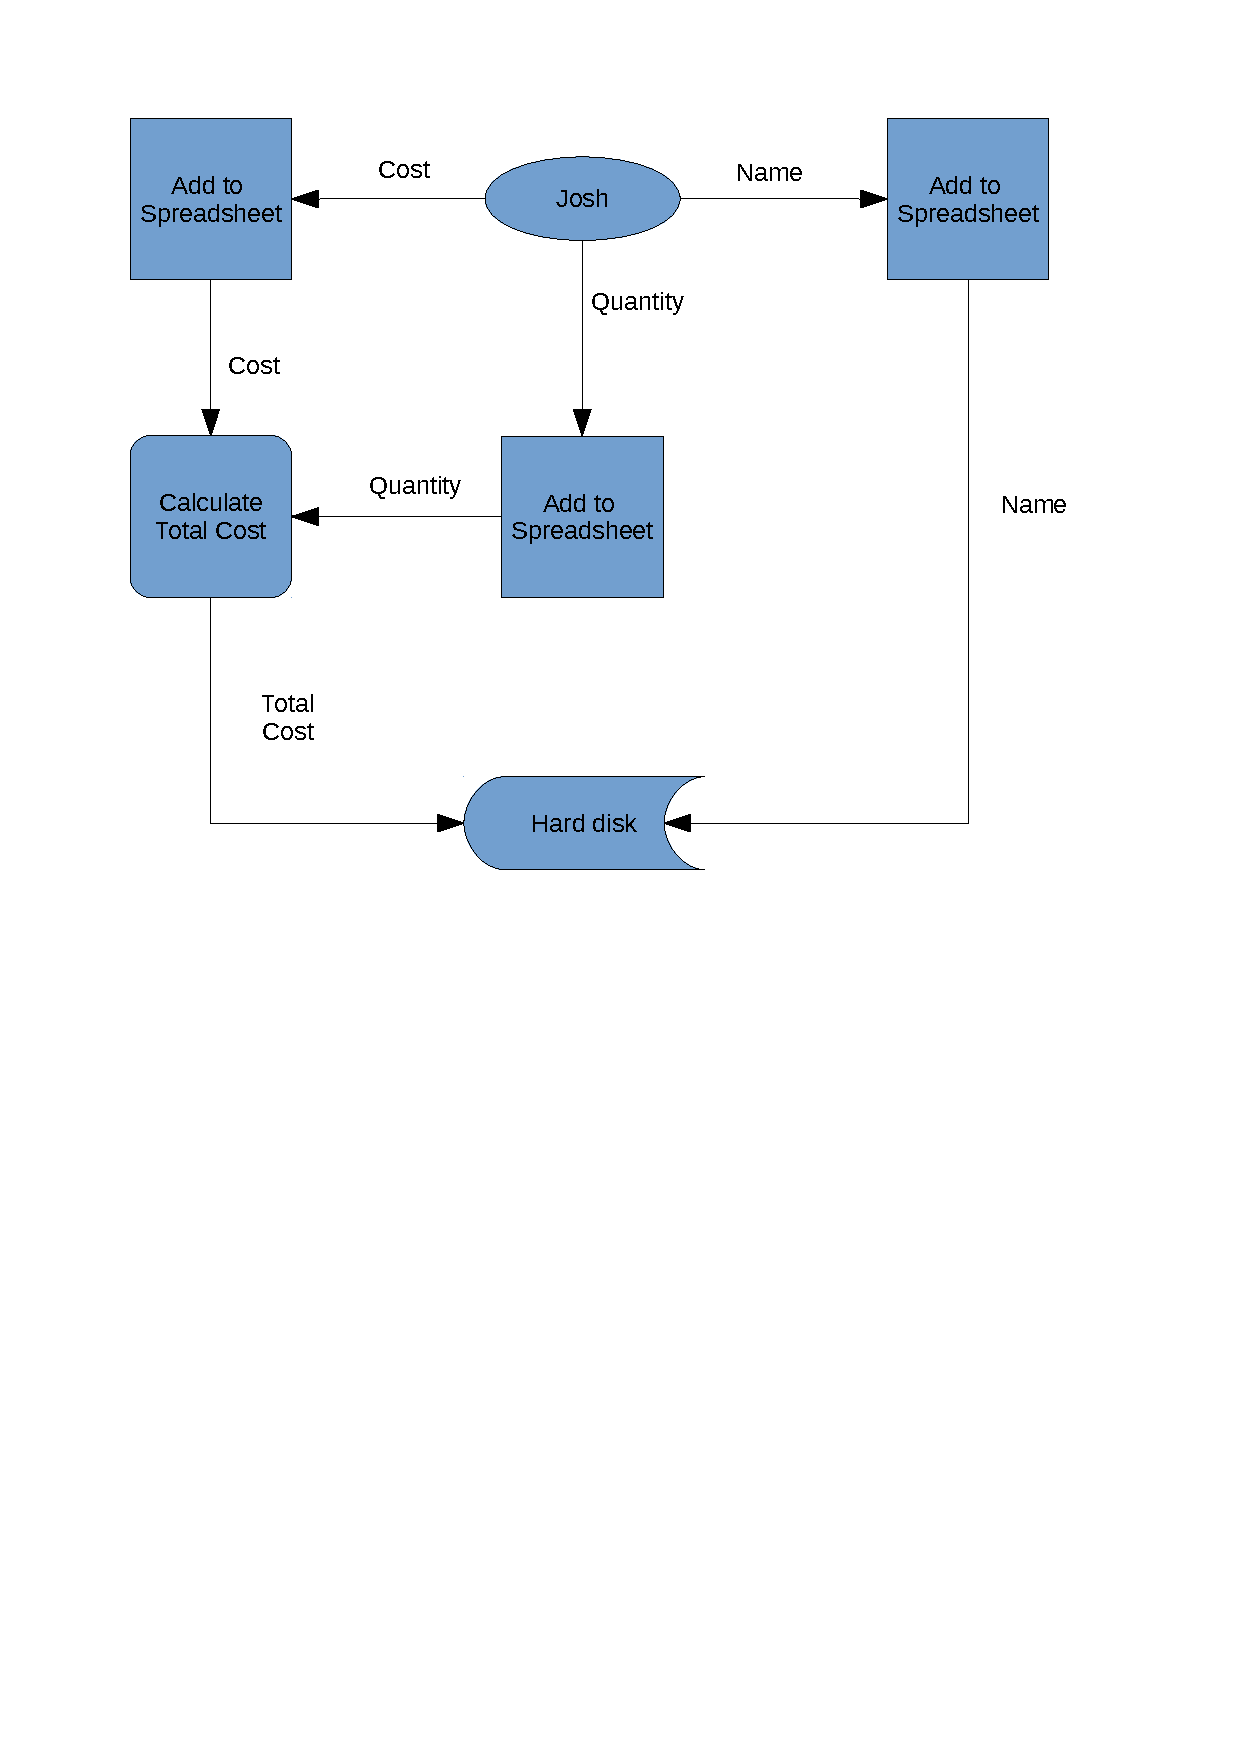
\includegraphics[width=\textwidth]{./Dataflow/Data_flow_new.pdf}
\end{figure}

\begin{figure}[H]
    \caption{Enter New Item.} \label{fig:print_function_result}
    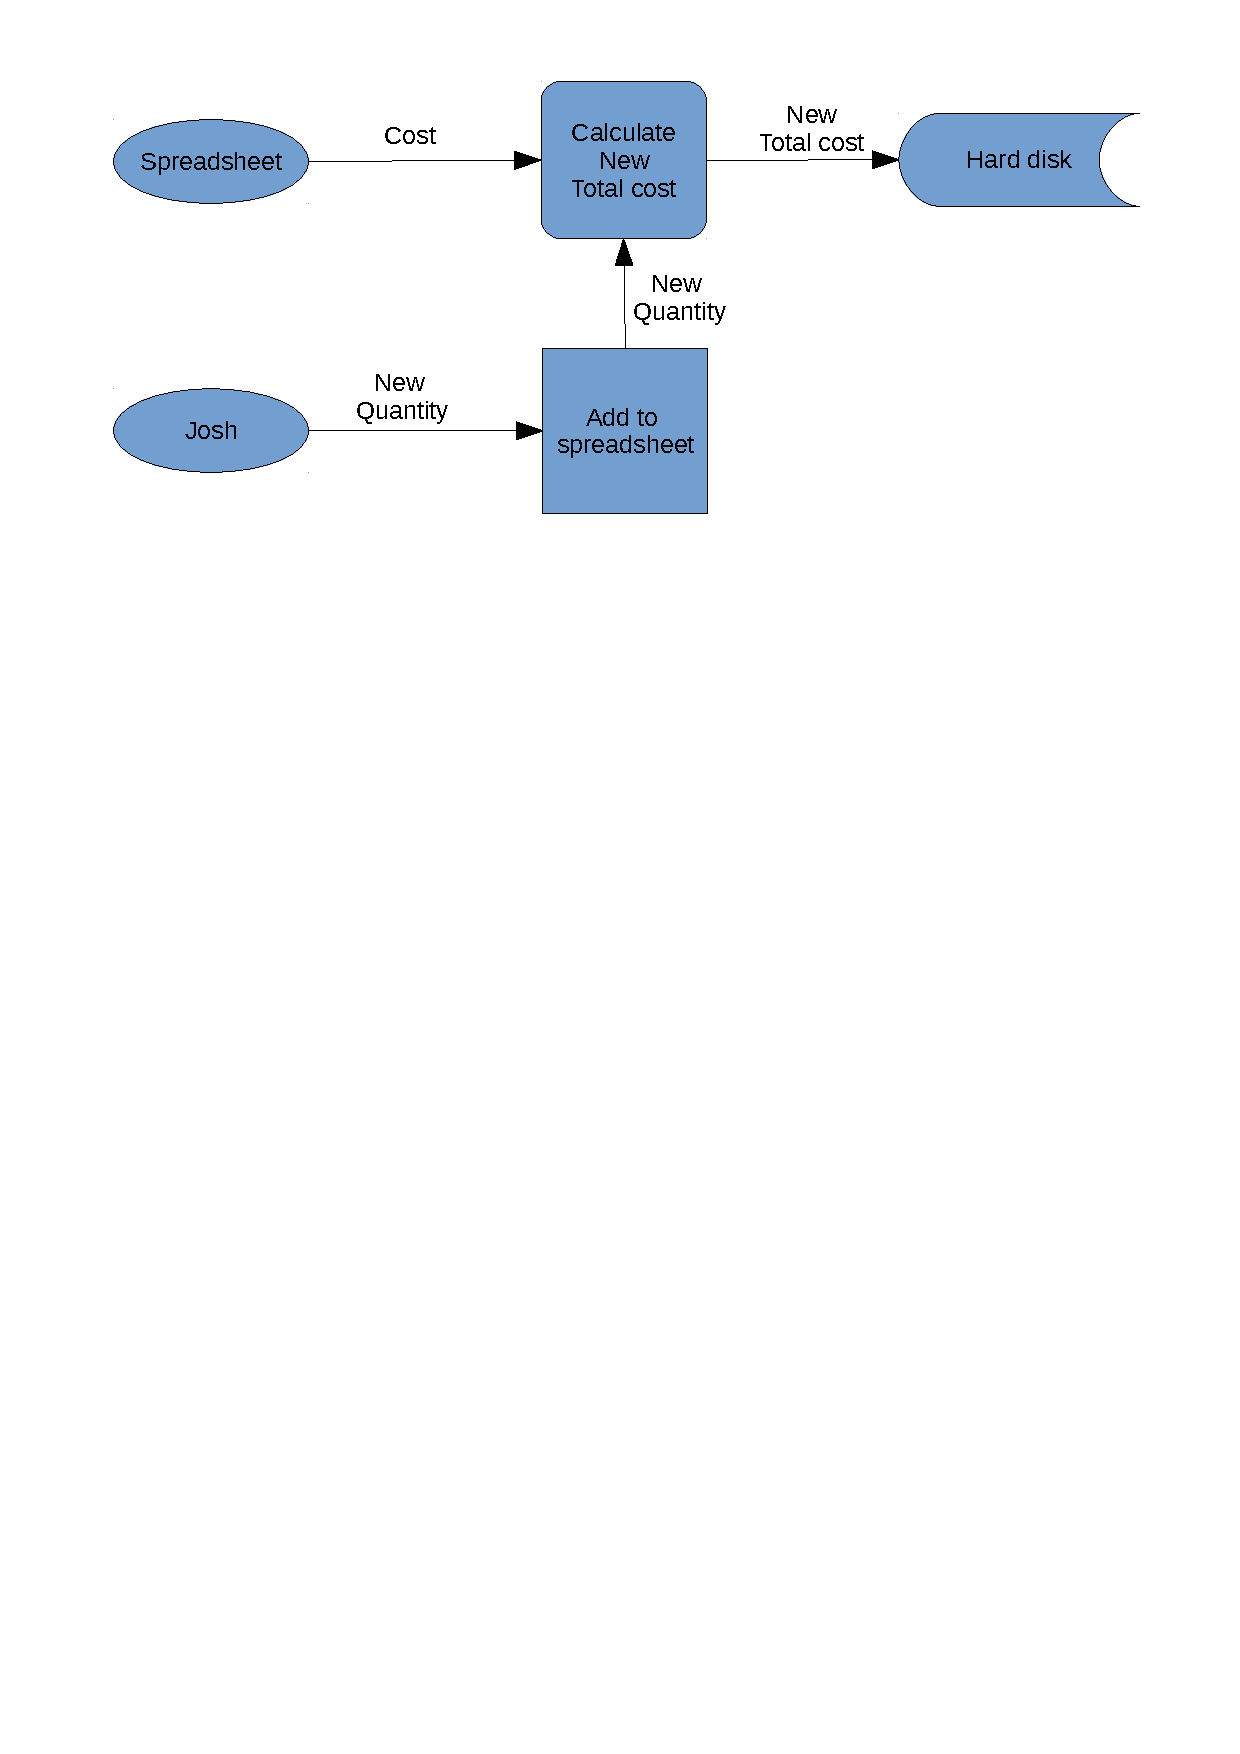
\includegraphics[width=\textwidth]{./Dataflow/Data_flow_update.pdf}
\end{figure}

\subsubsection{Data dictionary}

\begin{figure}[H]
    \caption{Data Dictionary.} \label{fig:data_dictionary}
    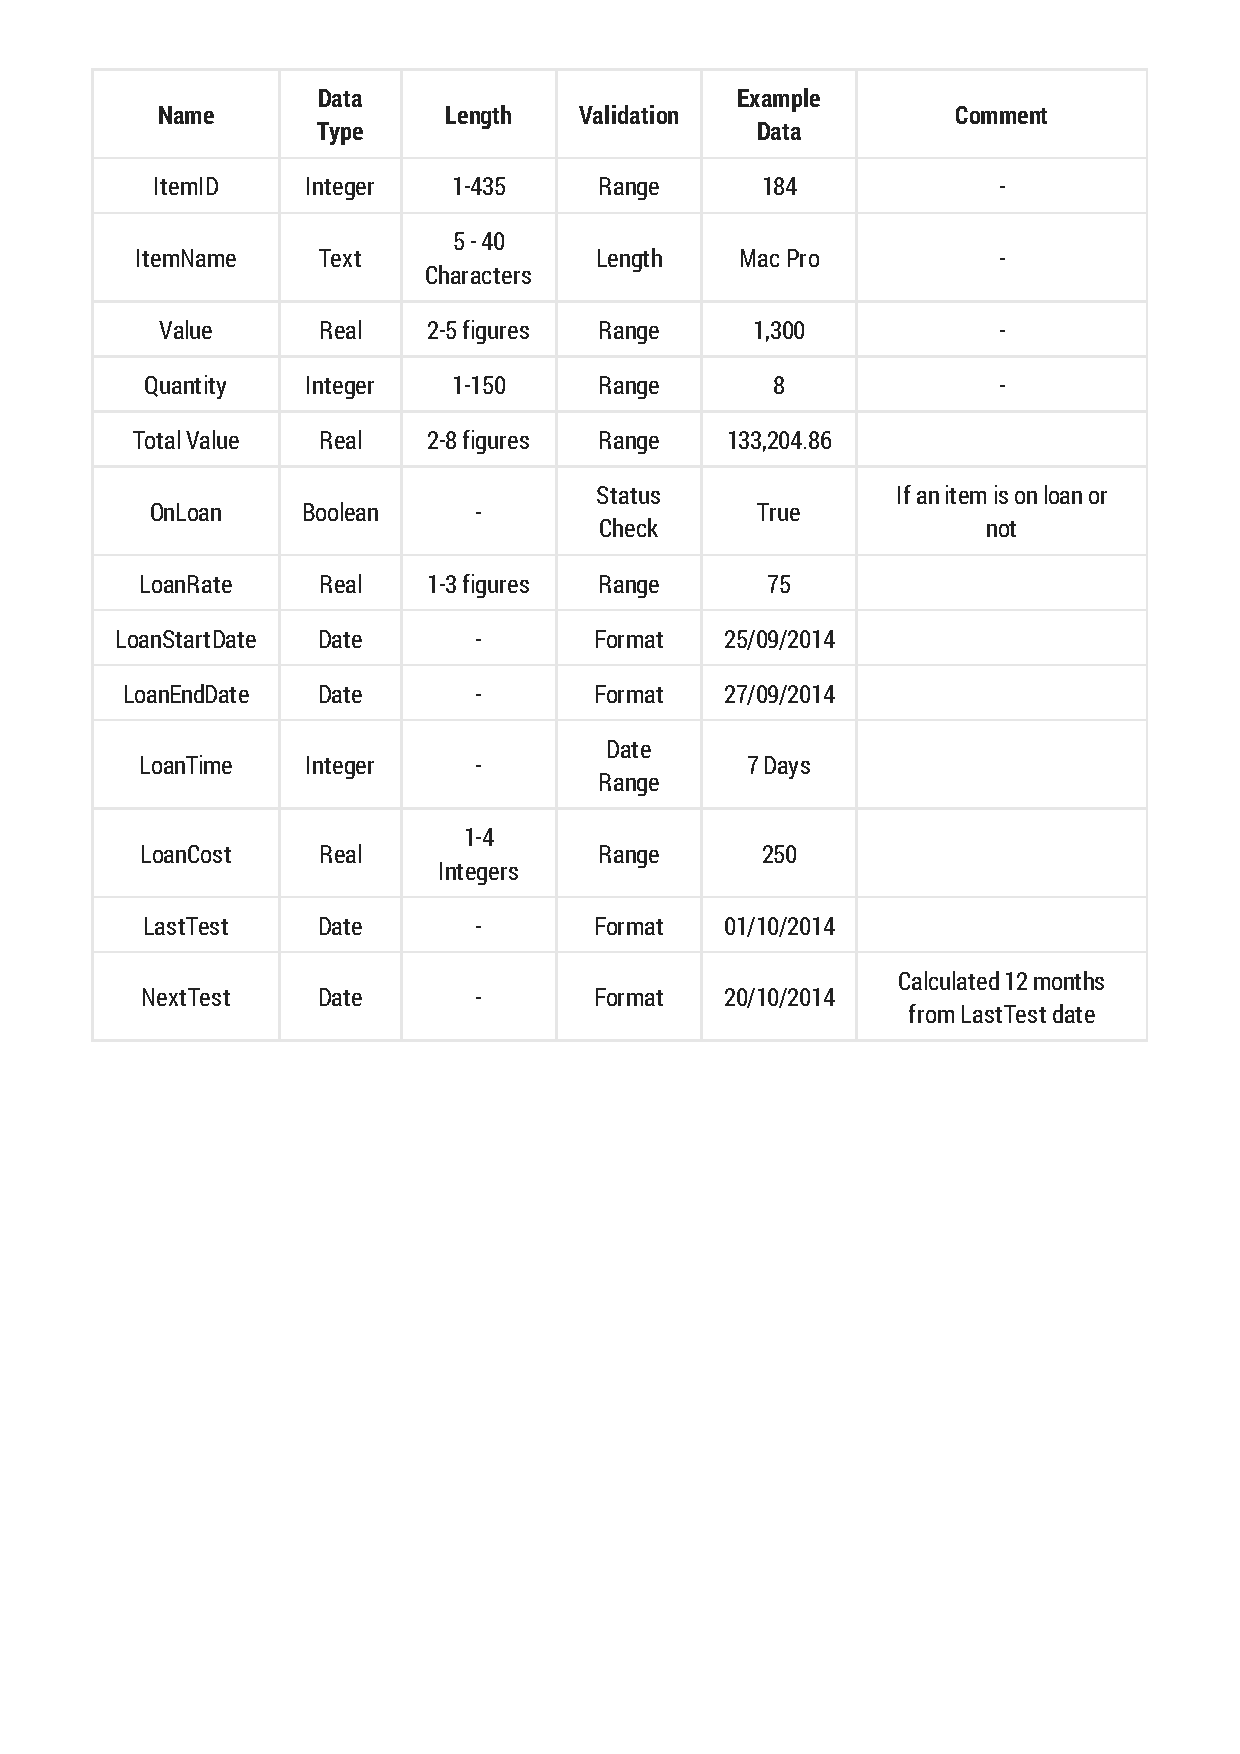
\includegraphics[width=\textwidth]{./Dictionary/Data_dictionary.pdf}
\end{figure}


\subsubsection{Volumetrics}

I have chosen to start off with only 20 Item Records along with 20 Loan Records and 20 PAT Test Records. In total there will be 60 Records.  I have chosen this number of records as my Client and I had previously agreed that this would be a suitable number of records to start with in order for him to get used to the system and train up other colleagues to know how to use it also. This can be increased as time goes by.

The Item Records Database, Loan Records Database and the PAT Test Records Database will store 18 fields of combined data. Each field should take up 1KB of hard disk space. With this the required initial storage space will be:

18KB * 60 = 1080KB

1080KB / 1024 = 1.05MB

If the rest of database managemnent system took up 28MB, the client would need 19.05MB of space for 60 records, with 18 fields of data

\newpage

\section{Objectives}

\subsection{General Objectives}

\begin{itemize}
	\item Easily understandable layout and structure for records.
	\item Easy structure for input and outputs.
	\item Easy viewing of records
\end{itemize}

\subsection{Specific Objectives}

Record viewing:
\begin{itemize}
    \item Clear labels for data attributes.
    \item Next and Preious record buttons.
    \item Edit button so data cannot be changed accidentally.
    \item Submit button to save data changes (if any) to the current record.
    \item First and Last record buttons to jump to respective record.
\end{itemize}

\noindent Data input:
\begin{itemize}
    \item Data fields become editable
    \item Drop down selection for location selection
    \item Changes saved immediately after editng has finished (ie submit button pressed)
\end{itemize}

\noindent Data output:
\begin{itemize}
    \item Print button and functionality
    \item Export records to PDF
    \item Print/Export a batch of records to PDF
\end{itemize}


\subsection{Core Objectives}

\begin{itemize}
    \item Viewing of Item/Loan/PAT-test Records
    \item Item/Loan/PAT-test data input
    \item Item/Loan/PAT-test data editing
    \item Sending of Loan Invoices
\end{itemize}

\subsection{Other Objectives}

\begin{itemize}
    \item Printing records/invoices
    \item Exporting records/invoices to PDF
\end{itemize}

\section{ER Diagrams and Descriptions}

\subsection{ER Diagram}

\begin{figure}[H]
    \caption{ER Diagrams.} \label{fig:ER Diagrams}
    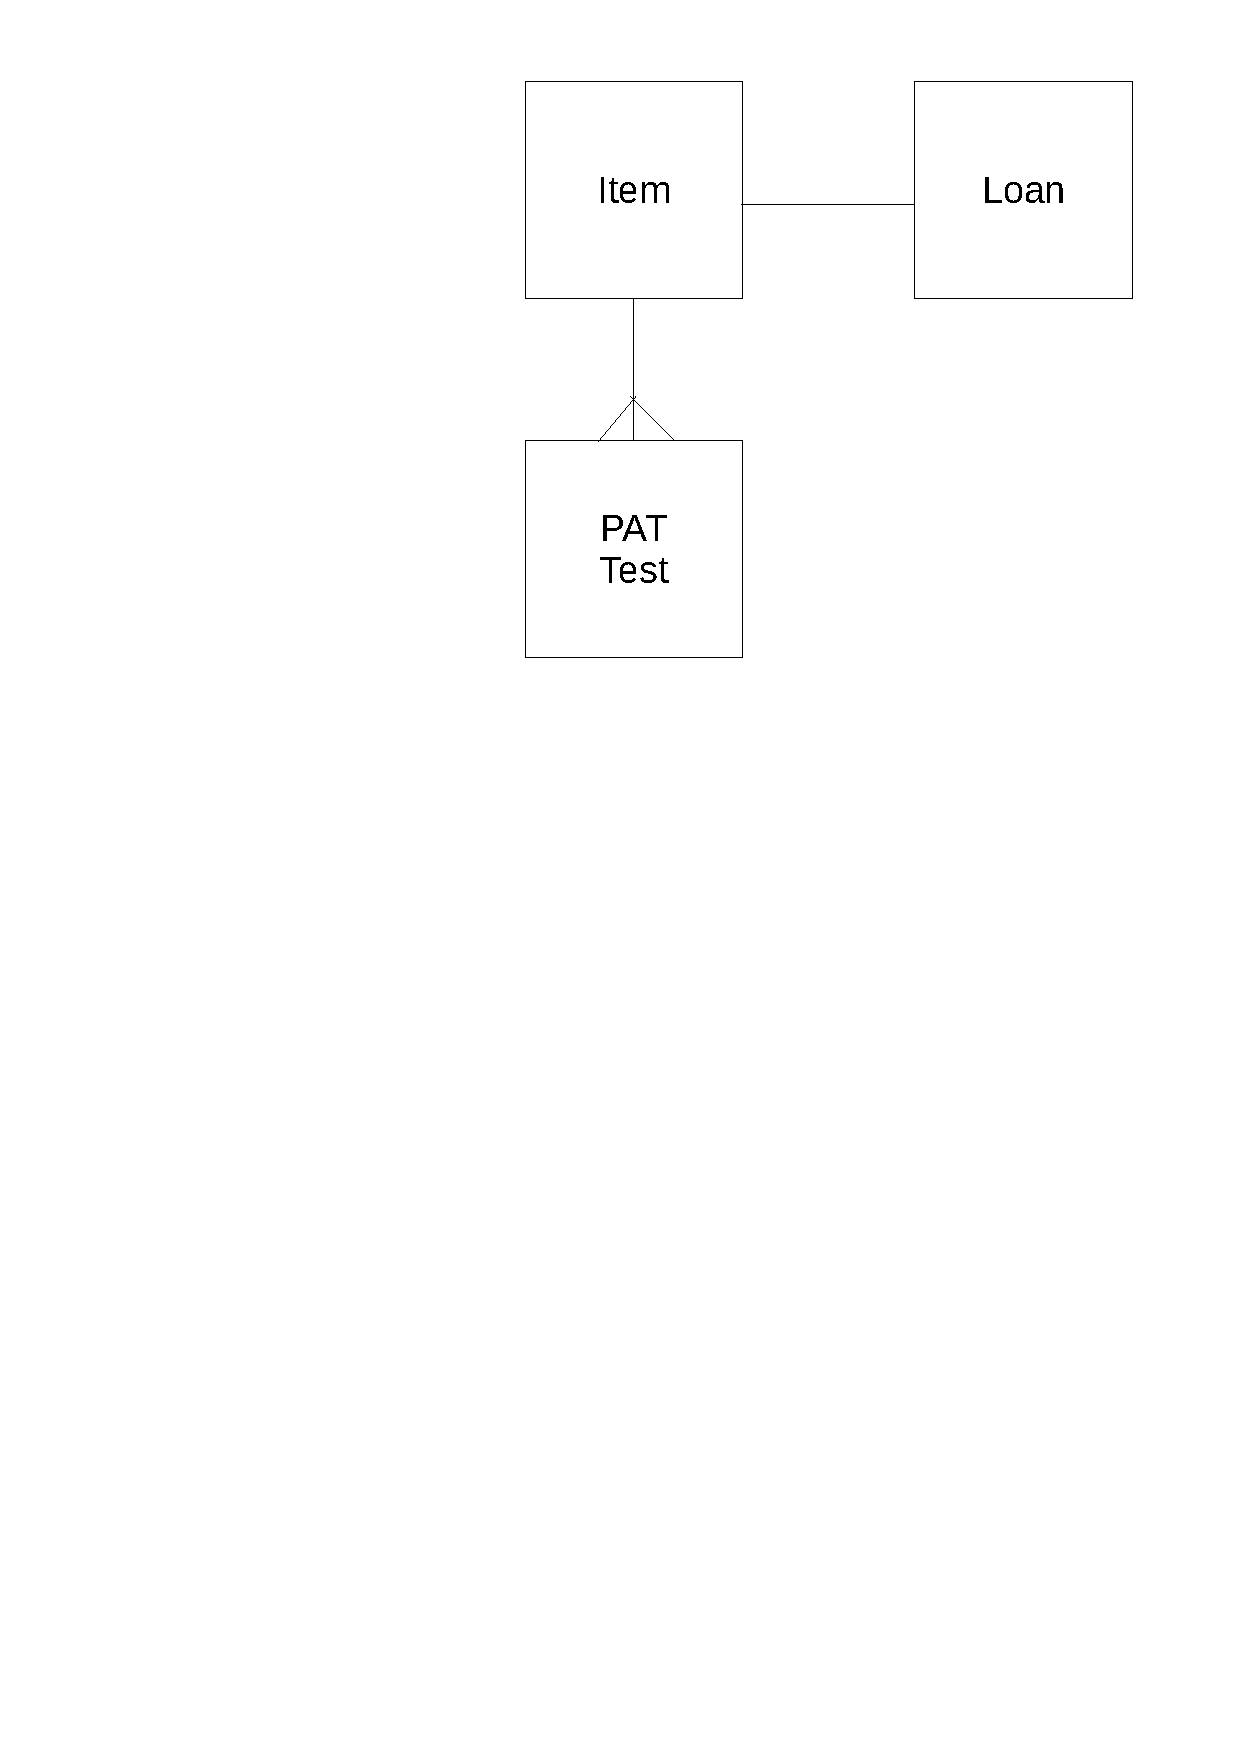
\includegraphics[width=\textwidth]{./ER_Diagrams/ER_Diagrams.pdf}
\end{figure}

\subsection{Entity Descriptions}

Item(\underline{ItemID},Name,Location,Value,Quantity,SubTotal,OnLoan, \emph{PATNeeded})

Loan(\underline{LoanID},\emph{ItemID},\emph{ItemName},LoanRate,LoanStartDate,LoanEndDate,LoanTime,LoanCost)

PATTest(\underline{TestID},\emph{ItemID},\emph{ItemName},LastTest,NextTest)

\section{Object Analysis}

\subsection{Object Listing}

\begin{itemize}
    \item Client
    \item Item
    \item Loan
    \item PAT test
\end{itemize}

\subsection{Relationship diagrams}

\subsection{Class definitions}

\section{Other Abstractions and Graphs}

\section{Constraints}

\subsection{Hardware}

\subsection{Software}

\subsection{Time}

\subsection{User Knowledge}

\subsection{Access restrictions}

\section{Limitations}

\subsection{Areas which will not be included in computerisation}

\subsection{Areas considered for future computerisation}

\section{Solutions}

\subsection{Alternative solutions}

\subsection{Justification of chosen solution}

\end{document}